\section{Theorie}
\label{sec:Theorie}

    Bei einem Operationsverstärker (OPV) handelt es sich um einen gleichstromgekoppelten Differenzverstärker.
    Das Schaltsymbol eines OPV ist in Abbildung \ref{fig:opv} dargestellt.
    Die Verstärkung der Differenz zwischen den beiden Eingangssignalen ergibt sich aus der
    Proportionalität zur Ausgangsspannung $U_A$:
    \begin{align}
        U_A = V(U_P - U_N) 
    \end{align}
    Wie in Abbildung \ref{fig:aussteu} zu sehen, ist diese Proportionalität nur für
    \begin{align}
        -U_B < U_A < U_B
    \end{align}
    gültig. Dieser Bereich wird als Aussteuerungsbereich bezeichnet. Verlässt die Ausgangsspannung dieses Intervall, ergibt sich eine S\"attigung und
    $U_A$ l\"auft gegen $\pm U_B$.

    \begin{figure}
    \centering
    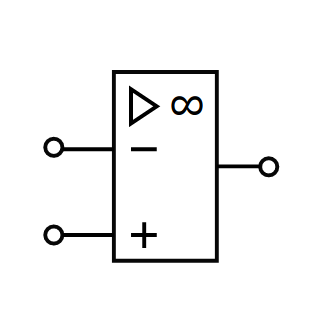
\includegraphics[width=0.4\textwidth]{Pics/schaltsymbol.png}
    \caption{Das Schaltsymbol für einen Operationsverstärker \cite{anleitungneu}.}
    \label{fig:opv}
    \end{figure}

    \begin{figure}
    \centering
    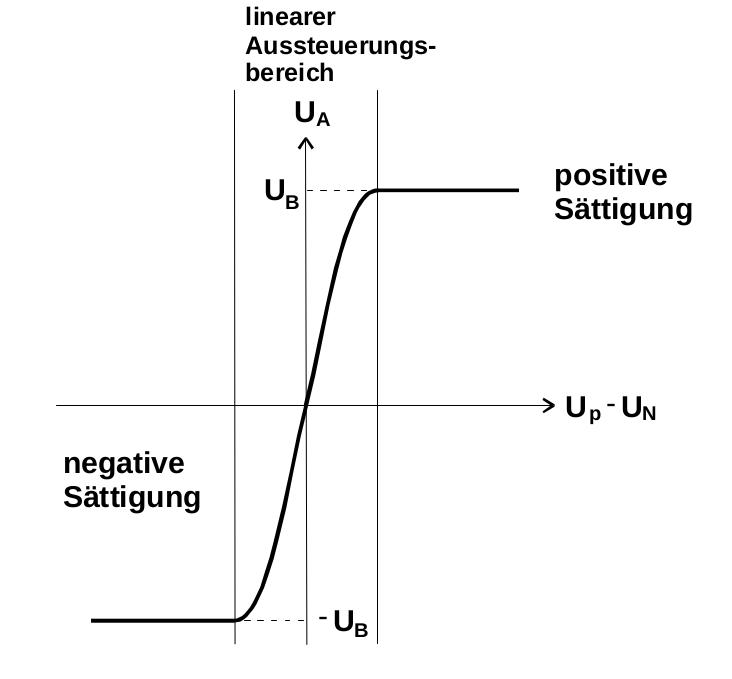
\includegraphics[width=0.4\textwidth]{Pics/aussteuerungsbereich.png}
    \caption{Die Kennlinie eines Operationsverstärkers \cite{anleitungalt}.}
    \label{fig:aussteu}
    \end{figure}

    Die Ausgangsspannung $U_A$ ist in Phase mit $U_P$ der als nicht-invertierender Eingang ("+"-Eingang) bezeichnet wird und Gegenphasig mit $U_N$, der invertierende Eingang ("-"-Eingang).
    Zur Veranschaulichung von Schaltungen mit OPV, wird die Idee eines idealen OPV eingeführt. Dieser ideale OPV hat im Gegenzug zum realen OPV folgende Eigenschaften:
    Eine unendlich hohe Leerlaufverstärkung $V_{\mathrm{id}}=\infty$, unendliche hohe Widerstände an den Eingängen, sowie einen Ausgangswiderstand von $r_a=0$.

    Bei einem realen OPV treten diverse Effekte auf, die in einem idealen OPV nicht existent sind.
    Einer dieser Effekte ist die Gleichtaktverstärkung
    \begin{align}
        V_{Gl} = \frac{\Delta U_A}{\Delta U_{Gl}},
    \end{align}
    die auftritt wenn die gleiche Spannung $U_{Gl}$ an den Eingängen liegt.
    Zusätzlich treten aufgrund der endlichen Eingangswiderstände ein Eingangsruhestrom
    \begin{align}
        I_B = \frac{1}{2}(I_P + I_N)
    \end{align}
    und ein Offsetstrom
    \begin{align}
        I_0 = I_P - I_N, U_P=U_N=0
    \end{align}
    auf.
    Zuletzt tritt bei einem realen OPV eine nicht verschwindende Ausgangsspannung auf wenn die Eingangspannungen gleich 0 gesetzt werden.
    Es wird der Begriff der Offsetspannung $U_0$ eingeführt
    \begin{align}
        U_0 = U_P - U_N,
    \end{align}
    welche die benötigte Differenz angibt damit $U_A$ verschwindet.
    Die Betrachtung des realen OPV geschieht durch Korrekturrechnungen an den Schaltungen mit einem idealen OPV.

    \subsection{Schaltungen mit Operationsverstärkern}
    \subsubsection{Invertierender-Linearverstärker}
    
    Um einen Operationsverstärker als Linearverstärker zu verwenden, wird ein Gegenkopplungszweig wie in Abb. \ref{fig:linear} verwendet.

    \begin{figure}
    \centering
    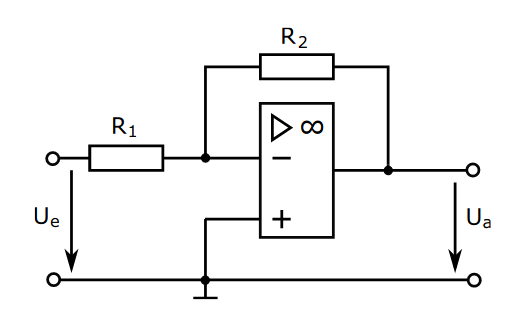
\includegraphics[width=0.6\textwidth]{Pics/linear.png}
    \caption{Die Schaltung für einen Invertierenden-Linearverstärker \cite{anleitungneu}.}
    \label{fig:linear}
    \end{figure}

    Es wird ein Teil der Ausgangsspannung auf den invertierenden Eingang gegeben. Dies führt zu einer Vergrößerung des Aussteuerungsbereich, wodurch auch höhere Eingangspannungen verwendet werden
    können ohne das eine Sättigung auftritt. Zudem erhöht die Verwendung einer Gegenkopplung die Stabilität der Verstärkung aufkosten des Verstärkungsgrades.
    Für die Verstärkung V' ergibt sich:
    \begin{align}
        V' = \frac{1}{V} + \frac{R_1}{R_2}.
    \end{align}
    Dabei steht $V$ f\"ur die Leerlaufverstärkung des Operationsverstärkers.
    Zuletzt führt eine Gegenkopplung zu einer Vergrößerung des Frequenzbandes, welches über den OPV übertragen werden kann (Abb. \ref{fig:frequenz}).

    \begin{figure}
    \centering
    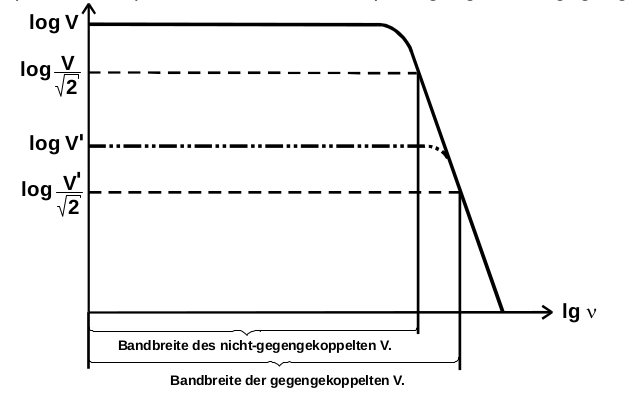
\includegraphics[width=0.6\textwidth]{Pics/frequenz.png}
    \caption{Die Frequenzgänge eines Linearverstärkers \cite{anleitungalt}.}
    \label{fig:frequenz}
    \end{figure}

    Diese Vergrößerung entspricht dabei einen Faktor
    \begin{align}
        g = \frac{V}{V'}.
    \end{align}

    Das Produkt aus Bandbreite und Verstärkung entspricht der Transitfrequenz, bei welcher die Verstärkung unabhängig von der Gegenkopplung auf den Wert 1 abfällt.

    \subsubsection{Umkehr-Integrator}

    Wird anstelle des einfachen Widerstandes in der Rückkopplung ein Kondesator eingebaut, ergibt sich die Schaltung in Abb. \ref{fig:integrator}.

    \begin{figure}
    \centering
    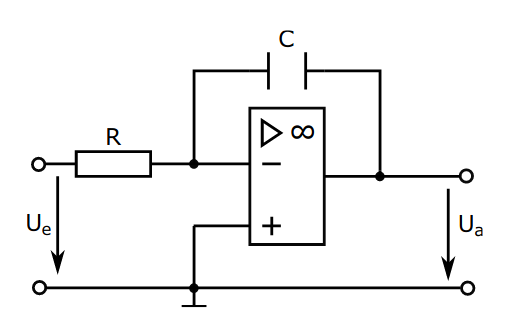
\includegraphics[width=0.6\textwidth]{Pics/integrator.png}
    \caption{Die Schaltung für einen Umkehr-Integrator \cite{anleitungneu}.}
    \label{fig:integrator}
    \end{figure}

    Dies führt zu einer Integration der Eingangspannung. Als Beispiel würde sich aus einer Eingangspannung $U_1 = U_0\sin(\omega t)$, die Ausgangsspannung
    $U_A = \frac{U_0}{\omega RC}\cos(\omega t)$ ergeben.
    Im Falle einer Sinusspannung würde daher die Ausgangsspannung mit $1/\omega$ abfallen.

    \subsubsection{Invertierender-Differenzierer}

    Ein tauschen des Widerstandes und Kondensators im Umkehr-Integrator führt zu der Schaltung in Abb. \ref{fig:diffdiff}. Dies wird als Invertierender-Differenzierer bezeichnet.

    \begin{figure}
    \centering
    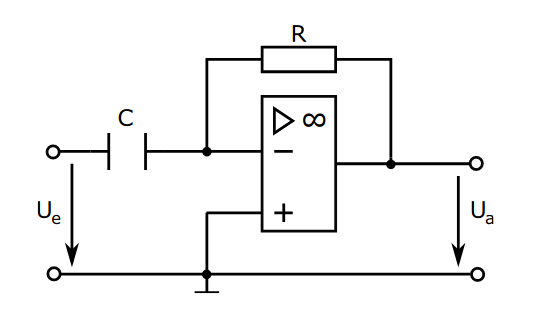
\includegraphics[width=0.6\textwidth]{Pics/diff.png}
    \caption{Die Schaltung für einen Invertierenden-Differenzierer \cite{anleitungneu}.}
    \label{fig:diffdiff}
    \end{figure}

    Diese Schaltung hat die Eigenschaft ein Eingangssignal zu differenzieren.
    Ein Eingangssignal der Form $U_1 = U_0\sin(\omega t)$ ergibt daher eine Ausgangsspannung $U_A = -\omega RCU_0\cos(\omega t)$, die proportional zu $\omega$ ist.

    \subsubsection{Nicht-Invertierender-Schmitt-Trigger}

    Eine weitere Schaltmöglichkeit mit einem OPV ist der Schmitt-Trigger, wie in Abb. \ref{fig:schmittimacschmitt} dargestellt.

    \begin{figure}
    \centering
    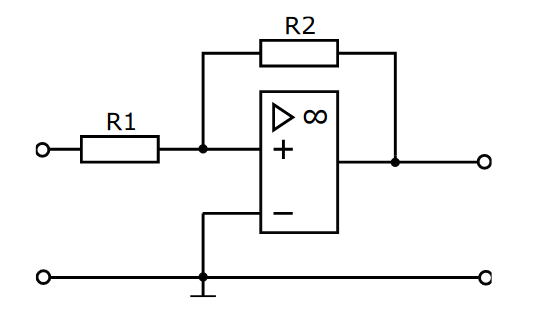
\includegraphics[width=0.6\textwidth]{Pics/schmitt.png}
    \caption{Die Schaltung für einen Nicht-Invertierenden-Schmitt-Trigger \cite{anleitungneu}.}
    \label{fig:schmittimacschmitt}
    \end{figure}

    Es wird durch die Mittkopplung ein Teil von $U_A$ auf die Eingangsspannung an den nicht-invertierenden Eingang gegeben. Dies f\"uhrt dazu dass eine Vergr\"o{\ss}erung der Ausgangsspannung eine Vergrößerung der
    Eingangspannung hervorruft, wodurch wiederum die Ausgangsspannung gr\"o{\ss}er wird.
    Die Schaltung zeigt dadurch ein instabiles Verhalten. Es ergibt sich eine Hystereseschaltung, in der $U_A$ auf den Wert $+U_B$ für $U_1\geq\frac{R_1}{R_2}U_B$ und $-U_B$ für $U_1\leq-\frac{R_1}{R_2}U_B$ springt.

    \subsubsection{Signalgenerator}

    Eine Zusammschaltung von Schmitt-Trigger und Umkehr-Integrator wie in Abb. \ref{fig:generator}, erschafft eine Möglichkeit Rechteck- und Dreiecksspannung zu generieren. Dafür wird die
    Schalteigenschaft des Schmitt-Triggers sowie die Integration des Ausgangssignal durch den Umkehr-Integrator verwendet. Die so erzeugten Signale sind in ihrer Frequenz von der Integratorkonstante und
    dem Teilerverhältnisse des Mitkopplungszweiges abhängig.

    \begin{figure}
    \centering
    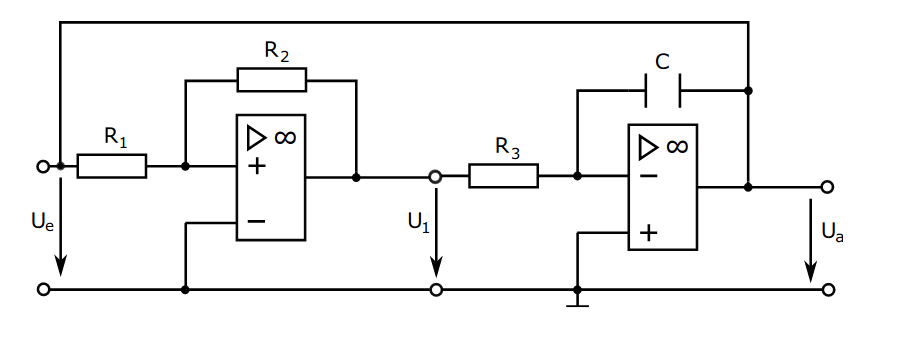
\includegraphics[width=0.6\textwidth]{Pics/generator.png}
    \caption{Die Schaltung für einen Signalgenerator \cite{anleitungneu}.}
    \label{fig:generator}
    \end{figure}

    \subsubsection{Variierende-Amplituden}

    Durch die in Abb. \ref{fig:varamp} dargestellt Schaltung lassen sich Sinusschwingungen mit zeitlich veränderlicher Amplitude generieren.

    \begin{figure}
    \centering
    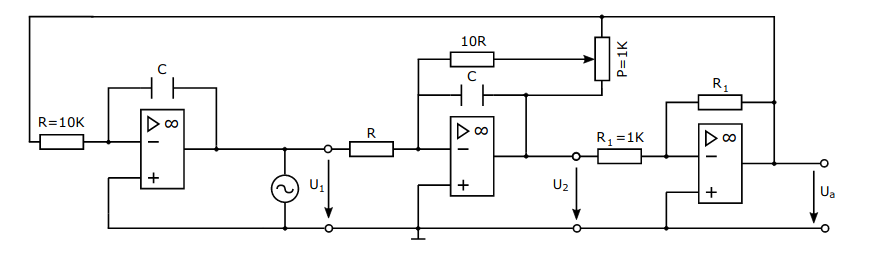
\includegraphics[width=1.2\textwidth]{Pics/varamp.png}
    \caption{Die Schaltung für einen Variierende-Amplitude \cite{anleitungneu}.}
    \label{fig:varamp}
    \end{figure}

    Aus der Schaltung lässt sich für die Ausgangsspannung folgende Differentialgleichung herleiten:
    
    \begin{align}
        \frac{\mathrm{d^2}U_A}{\mathrm{d}t^2} - \frac{\eta\mathrm{d}U_A}{10RC\mathrm{d}t} + \frac{U_A}{(RC)^2} = 0
    \end{align}
    Dabei steht $\eta$ für die Dämpfung ($\eta<0$) beziehungsweise Enddämpfung ($\eta>0$) des Systems.
    Der Gleichung genügt die Lösung
    \begin{align}
        U_A(t) = U_0\exp(\frac{\eta t}{20RC})\sin(\frac{t}{RC})
    \end{align}

    Es ergibt sich eine Schwingungsdauer von
    \begin{align}
        T = 2\pi RC.
    \end{align}
    Die Abklingsdauer, das heißt die Zeit bis die Amplitude auf den e-ten Teil gefallen ist, wird durch
    \begin{align}
        \tau = \frac{20RC}{|\eta|}
    \end{align}
    beschrieben.